\documentclass[10pt,lang=cn]{elegantpaper}

\usepackage{threeparttable}
\usepackage{ctex}
\usepackage{titlesec} %自定义多级标题格式的宏包
\usepackage{setspace} %设置单倍行距的宏包
\usepackage{makecell}
%图片并排需要的宏包
\usepackage{graphicx}
\usepackage{float} 
\usepackage{subfigure}
% Start of 'ignore natbib' hack
\let\bibhang\relax
\let\citename\relax
\let\bibfont\relax
\let\Citeauthor\relax
\let\textcite\relax
\makeatletter
\DeclareRobustCommand{\MakeUppercase}[1]{{%
      \def\i{I}\def\j{J}%
      \def\reserved@a##1##2{\let##1##2\reserved@a}%
      \expandafter\reserved@a\@uclclist\reserved@b{\reserved@b\@gobble}%
      \protected@edef\reserved@a{\uppercase{#1}}%
      \reserved@a
   }}
\DeclareRobustCommand{\MakeLowercase}[1]{{%
      \def\reserved@a##1##2{\let##2##1\reserved@a}%
      \expandafter\reserved@a\@uclclist\reserved@b{\reserved@b\@gobble}%
      \protected@edef\reserved@a{\lowercase{#1}}%
      \reserved@a
   }}
\makeatother
\expandafter\let\csname ver@natbib.sty\endcsname\relax
% End of 'ignore natbib' hack
\usepackage[citestyle=authoryear,bibstyle=numeric,sorting=nty]{biblatex}
\addbibresource{wpref.bib}

\setCJKmainfont[ItalicFont=仿宋,BoldFont=黑体]{仿宋}

\graphicspath{{figures/}}
% 设置字号命令
\newcommand{\sanhao}{\fontsize{16pt}{\baselineskip}\selectfont} %三号
\newcommand{\sihao}{\fontsize{14pt}{\baselineskip}\selectfont} %四号
\newcommand{\wuhao}{\fontsize{10.5pt}{\baselineskip}\selectfont} %五号
% 设置引用在右上角
\newcommand{\upcite}[1]{\textsuperscript{\textsuperscript{\cite{#1}}}}
% 设置章节编号格式
\titleformat{\section}[block]{\centering\sihao\kaishu}{\zhnum{section}}{0.5em}{}[] %一级标题用一、二、三等编号,标题占3行,4号楷体,居中
\titleformat{\subsection}[block]{\wuhao\fangsong\hspace{2em}}{(\zhnum{subsection})}{0.1em}{}[] %二级标题用(一)、(二)、(三)等编号,标题占2行,5号仿宋体,左空2格
\titleformat{\subsubsection}[block]{\wuhao\fangsong\hspace{2em}}{\arabic{subsubsection}.}{0.1em}{}[] %三级标题用1.、2.、3.等编号,标题占1行,5号仿宋体,左空2格
\titlespacing*{\subsubsection}{0pt}{2pt}{2pt} %设置三级标题占一行并为单倍行距
% 设置摘要字号大小为五号
\renewcommand{\abstractnamefont}{\wuhao\bfseries}

% 设置目录空格
\renewcommand{\contentsname}{\centering {目 \quad 录}}

\makeatletter
% 默认生成长度为4cm的下划线
\newcommand\dlmu[2][4cm]{\hskip1pt\underline{\hb@xt@ #1{\hss#2\hss}}\hskip3pt}
% 设置标题大小为三号
\patchcmd{\@maketitle}{\LARGE}{\sanhao}{}{}
\makeatother

% 标题信息
\title{这是一篇中央财经大学课程论文 \vspace{-2em}} %减少标题下方的空白
\date{}

\begin{document}

% 封面页
\begin{titlepage}
    \begin{center}
        \begin{figure}[!h]
            \centering
            
\includegraphics[width=.7\textwidth]{logo}
        \end{figure}
        
        \vspace*{80pt}

        \begin{tabular}{cc}
            \sihao \kaishu{学年学期:}&
            \sihao {\dlmu[8cm]{202x——202x学年第x学期}}\vspace{12pt}\\
            \sihao \kaishu{课程名称:}&
            \sihao {\dlmu[8cm]{你的课程名称}}\vspace{12pt}\\
            \sihao \kaishu{课程代码:}&
            \sihao {\dlmu[8cm]{0000000}}\vspace{12pt}\\
            \sihao \kaishu{任课教师:}&
            \sihao {\dlmu[8cm]{王xx \ 李xx}}\vspace{12pt}\\
            \sihao \kaishu{姓 \qquad   名:}&
            \sihao {\dlmu[8cm]{你的名字}}\vspace{12pt}\\
            \sihao \kaishu{学 \qquad   号:}&
            \sihao {\dlmu[8cm]{202x123456}}\vspace{12pt}\\
            \sihao \kaishu{班  \qquad  级:}&
            \sihao {\dlmu[8cm]{你的班级}}\vspace{40pt}\\

            \sihao \kaishu{总 \qquad   分:}&
            \sihao {\dlmu[8cm]{}}\vspace{12pt}\\
            \sihao \kaishu{评 \hfill 分 \hfill 人:}&
            \sihao {\dlmu[8cm]{}}
        \end{tabular}
        
    \end{center}

    \clearpage

\end{titlepage}

\maketitle

% \tableofcontents
% \newpage
\pagenumbering{arabic} %罗马数字页码

\begin{abstract}
    \linespread{0.91} %设置单倍行距
    \wuhao\fangsong %设置字体和字号
    \indent 这是摘要
\keywords{\fangsong{关键词1\quad 关键词2\quad 关键词3}}
\end{abstract}

\begin{spacing}{1.06} %设置正文单倍行距
    \wuhao %设置字号
\section{引言}

让我们试试第一种引用\parencite{peterson2017role}

\section{文献综述}

\subsection{这是一个小节}

\Citeauthor{peterson2017role}在\citeyear{peterson2017role}年的研究中发现了一些奇妙的现象。

\subsection{这是另一个小节}

让我们试试插入图像。如图\ref{fig:test}所示

\begin{figure}[!h]
    \centering
    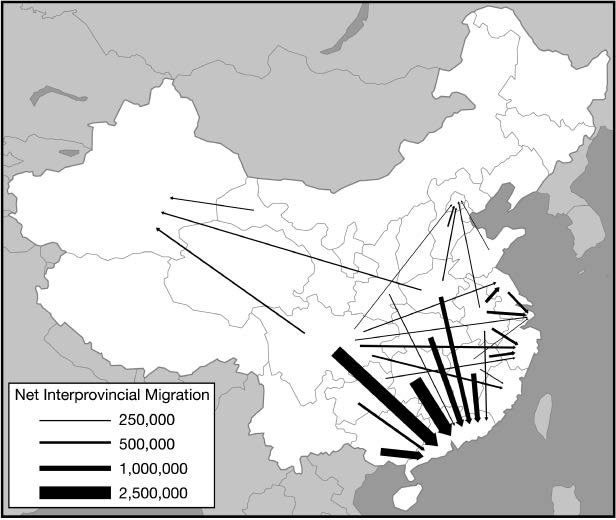
\includegraphics[width=.6\textwidth]{test}
    \caption{这是一个测试图像}
    \label{fig:test}
\end{figure}

让我们试试另一种引用。
\textcite{chaurasia2021economic}分析了奇妙的问题。

\end{spacing}

\printbibliography[title={参考文献}]

\end{document}